\documentclass[tikz,dvipsnames]{standalone}
\usepackage[utf8]{inputenc}
\usepackage[]{xcolor}
\PassOptionsToPackage{dvipsnames}{xcolor}
\usepackage{amsmath}
\usepackage{amssymb}

\usetikzlibrary{arrows,positioning,shapes}
\usetikzlibrary{decorations.pathreplacing,decorations.markings}
\usetikzlibrary{calc}
% https://tex.stackexchange.com/questions/3161/tikz-how-to-draw-an-arrow-in-the-middle-of-the-line
\tikzset{
  % style to apply some styles to each segment of a path
  on each segment/.style={
    decorate,
    decoration={
      show path construction,
      moveto code={},
      lineto code={
        \path [#1]
        (\tikzinputsegmentfirst) -- (\tikzinputsegmentlast);
      },
      curveto code={
        \path [#1] (\tikzinputsegmentfirst)
        .. controls
        (\tikzinputsegmentsupporta) and (\tikzinputsegmentsupportb)
        ..
        (\tikzinputsegmentlast);
      },
      closepath code={
        \path [#1]
        (\tikzinputsegmentfirst) -- (\tikzinputsegmentlast);
      },
    },
  },
  % style to add an arrow in the middle of a path
  mid arrow/.style={postaction={decorate,decoration={
        markings,
        mark=at position .5 with {\arrow[#1]{stealth}}
      }}},
  % style to add an arrow at a position of a path
  arrow at/.style 2 args={postaction={decorate,decoration={
        markings,
        mark=at position #1 with {\arrow[#2]{stealth}}
      }}},
}

\tikzset{cross/.style={cross out, draw=black, minimum size=2*(#1-\pgflinewidth), inner sep=0pt, outer sep=0pt},
%default radius will be 1pt. 
cross/.default={1pt}}

%color
\colorlet{TopOp1}{RedOrange}
\colorlet{TopOp2}{JungleGreen!60!black}
\colorlet{TopOp3}{Mulberry}

\usetikzlibrary{knots}
\begin{document}
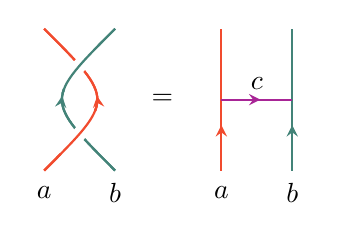
\begin{tikzpicture}[thick,scale=1.5]
  \pgfmathsetmacro{\wid}{.6}
  \pgfmathsetmacro{\ll}{.6}
  \begin{knot}[
    %draft mode=crossings,
    clip width=2.5,
    flip crossing=2]
    \strand[color=TopOp1,draw,] (0,-\ll) .. controls (\wid,0) .. (0,\ll) ;
    \strand[color=TopOp2,draw,] (\wid,-\ll) .. controls (0,0).. (\wid,\ll) ;
  \end{knot}
  \draw[color=TopOp1,draw=none,arrow at={.52}{}] (0,-\ll) .. controls (\wid,0) .. (0,\ll) ;
  \draw[color=TopOp2,draw=none,arrow at={.52}{}] (\wid,-\ll) .. controls (0,0).. (\wid,\ll) ;
  \node[yshift=-8] at (0,-\ll) {$a$};
  \node[yshift=-8] at (\wid,-\ll) {$b$};

  \begin{scope}[xshift=1.5cm]
  \draw[color=TopOp1,arrow at={.32}{}] (0,-\ll) -- (0,0) coordinate(ml) -- (0,\ll) ;
  \draw[color=TopOp2,arrow at={.32}{}] (\wid,-\ll) -- (\wid,0) coordinate(mr) -- (\wid,\ll) ;
  \node[yshift=-8] at (0,-\ll) {$a$};
  \node[yshift=-8] at (\wid,-\ll) {$b$};
  \draw[arrow at={.55}{},color=TopOp3] (ml) -- (mr);
  \node[anchor=south] at ($(ml)!.5!(mr)$){$c$};
  \node at (\wid+.1,0){};
  \node at (-.5,0) {$=$};
  \end{scope}
\end{tikzpicture}
\end{document}
